\chapter{Transferring Files}

\section{Transferring Files}
\label{cha:transferring-files}
\index{SD Cards!Transferring Files}

While there is plenty of fun to be had writing your own programs for the MEGA65, eventually you will want to run programs written by others. You may also want to back up your MEGA65 programs to your PC for safe keeping.

You can copy D81 virtual disk images to your MEGA65-formatted SD card using any PC, without any special tools or software. Your PC will recognize the data region of the SD card as a FAT32 partition. If you use this method, be aware that some PC operating systems may have unwanted side effects, such as fragmentation of SD card files, or extraneous files created by macOS Finder. These effects are harmless to the data, but may require maintenance to keep the card useful in the MEGA65.\footnote{If the MEGA65 reports a fragmented file, you can use a PC disk defragmentation tool on the data partition. Alternatively, you can copy all files off of the SD card to the PC, re-format the SD card in the MEGA65, then copy the files back from the PC.}

The fastest and most reliable way to transfer files between your PC and your MEGA65 is with an Ethernet cable.\index{Networking!Ethernet} You connect one end of the cable to the RJ45 jack on the rear of the MEGA65. You can connect the other end to your local area network (LAN) router or switch, or connect it directly to your PC. You use software on your PC to initiate file transfers, in either direction: from the PC to the MEGA65, or from the MEGA65 to the PC.

It is also possible to transfer files using a JTAG or UART Serial interface connected to the main board. This is an advanced technique and is not described in this User's Guide. Most people will prefer the Ethernet method.\footnote{JTAG or UART Serial hardware provides access to a debugging interface that may be useful to some programmers. JTAG is also useful for developing FPGA cores. For more information, see {\it MEGA65 Developer's Guide.}}

\section{Understanding Networking}

The MEGA65 can use Ethernet to connect to or accept connections from other computers on a network. With appropriate software, it can connect to other computers over the Internet.

The MEGA65 Ethernet hardware presents a Media Access Control (MAC) address to the local network.\index{Networking!MAC address} Unlike other Ethernet hardware, the MEGA65's MAC address is not assigned at the factory: it is set in the Configuration Utility. (See chapter \vref{cha:configuringyourmega}.)

For file transfers, you instruct the MEGA65 to listen for incoming connections, then use M65Connect (or another tool, such as \texttt{mega65\_ftp}) on your PC to initiate a connection. The tool assigns an IP address to the MEGA65 that is an address on your local network. You will need to know your local network's valid range of IP addresses to determine an appropriate address for the MEGA65. A typical home router establishes a local network with addresses such as \texttt{192.168.0.x}, where \texttt{x} is a number in the range 2 -- 254. One possible local IP address for the MEGA65 on such a network might be \texttt{192.168.0.65}.

% TODO: Our tools may eventually involve DHCP in the automatic selection of an IP address for the MEGA65.

Modern computers typically use the Dynamic Host Configuration Protocol (DHCP) to obtain an IP address from the local router. The MEGA65 network listener does not support DHCP. You will need to configure your router to prevent the IP address that you select for the MEGA65 from being assigned to another computer. See your router's documentation for information on how to do this. (It is possible to avoid this step if no other computer on your network is assigned to the address you pick, but it's best to not leave this to chance.)

Most local network routers are configured to block incoming connections originating from the Internet (a ``firewall''). This is an important safety precaution in general. This is especially important for the MEGA65, because the MEGA65 network listener has no security protections of its own. {\em Do not configure your network router to allow incoming connections to reach the MEGA65 when using the network listener feature described below.}

% TODO: more info on how to pick an IP address based on a direct Ethernet connection

As an alternative to connecting the MEGA65 to your local network, if your PC has an Ethernet jack, you can connect your MEGA65 directly to your PC via Ethernet. In this case, the IP address of the MEGA65 can be any valid address compatible with your PC's network configuration.

\section{Obtaining the File Transfer Tools}
\index{M65Connect Application}

{\bf M65Connect} is an application for Windows, Mac, or Linux that facilitates file transfers and other useful features for MEGA65 users. The application has a windowed interface, and also includes command-line tools useful for programming.

To obtain M65Connect:

\begin{enumerate}
\item Visit the MEGA65 Filehost website\index{Filehost website} in a browser: \url{https://files.mega65.org}
\item In the search box in the top right corner, type: ``M65Connect''
\item Select the version of M65Connect for your PC operating system.
\item Click the ``Download'' button.
\item Use your PC to unpack the downloaded archive file.
\end{enumerate}

\subsection{M65Connect for Windows}

The Windows version of M65Connect is in the ``M65Connect'' folder: {\bf M65Connect.exe}. As with most open source software, Microsoft Defender may refuse to run the software, displaying a dialog window. If this happens, click ``More info,'' then click the ``Run anyway'' button that appears.

The command-line tools are in a sub-folder named ``M65Connect Resources,'' such as: {\tt M65Connect Resources\textbackslash{}mega65\_ftp.exe}

\subsection{M65Connect for macOS}

The macOS version of M65Connect is a Mac application bundle: {\bf M65Connect.app}. As with most open source software, macOS does not recognize it as ``signed'' by the developer, and macOS will refuse to run it. To run the application for the first time:

\begin{enumerate}
\item Right-click on the {\bf M65Connect.app} icon. In the pop-up menu, select ``Open.'' A dialog will open.
\item Click the ``Open'' button. The application will open.
\end{enumerate}

On subsequent runs, you can double-click the icon as with any other application.

The command-line tools are inside the application bundle directory, such as: {\tt M65Connect.app/Contents/mega65\_ftp.osx}

\subsection{M65Connect for Linux}

The Linux version of M65Connect is in the ``M65Connect'' folder: {\bf M65Connect}. Double-click it to run.

The command-line tools are in a sub-folder named ``M65Connect Resources,'' such as: {\tt M65Connect Resources/mega65\_ftp}

\section{Enabling Network Listening}
\index{Networking!Network Listening Mode}

By default, the MEGA65 ignores all attempts by other computers to connect to it over the network. Software running on the MEGA65 can listen for network connections, but the MEGA65 does not do this on its own.

To transfer files with M65Connect, you must set the MEGA65 to listen for incoming connection attempts from M65Connect. This requires two steps:

\begin{itemize}
\item Set the DIP switch \#2 on the main board to the ``on'' position.
\item Enable a network listening session by pressing this key combination: \specialkey{SHIFT} + \megakey{\pounds}
\end{itemize}

To set the DIP switch,\index{DIP switches} open the case, as described in \vref{cha:setup}. Locate the DIP switches on the main board, then set DIP switch \#2 to the ``on'' position.

\begin{center}
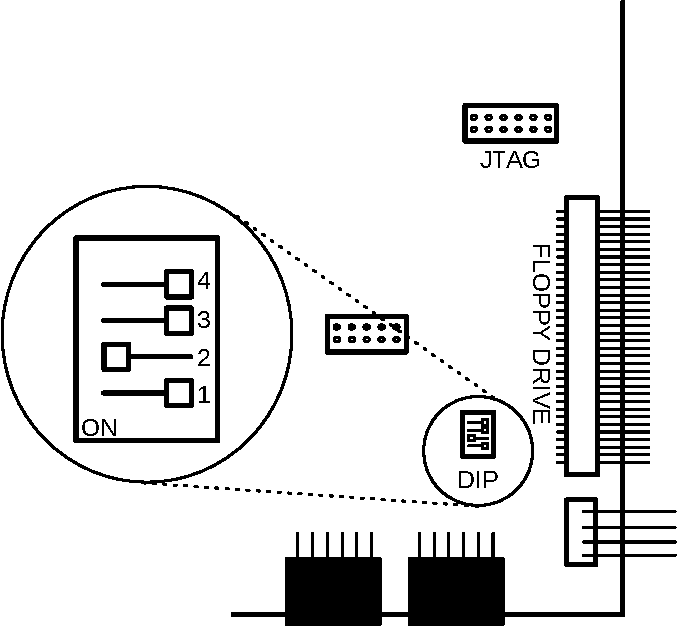
\includegraphics[width=\linewidth]{images/illustrations/mega65-dip2.pdf}
\end{center}

It is safe to leave DIP \#2 in this position for regular operation. It is set to off at the factory to avoid accidental activation.

To enable a network listening session, press \specialkey{SHIFT} + \megakey{\pounds}. The power light blinks between yellow and green when network listening is active.

\begin{center}
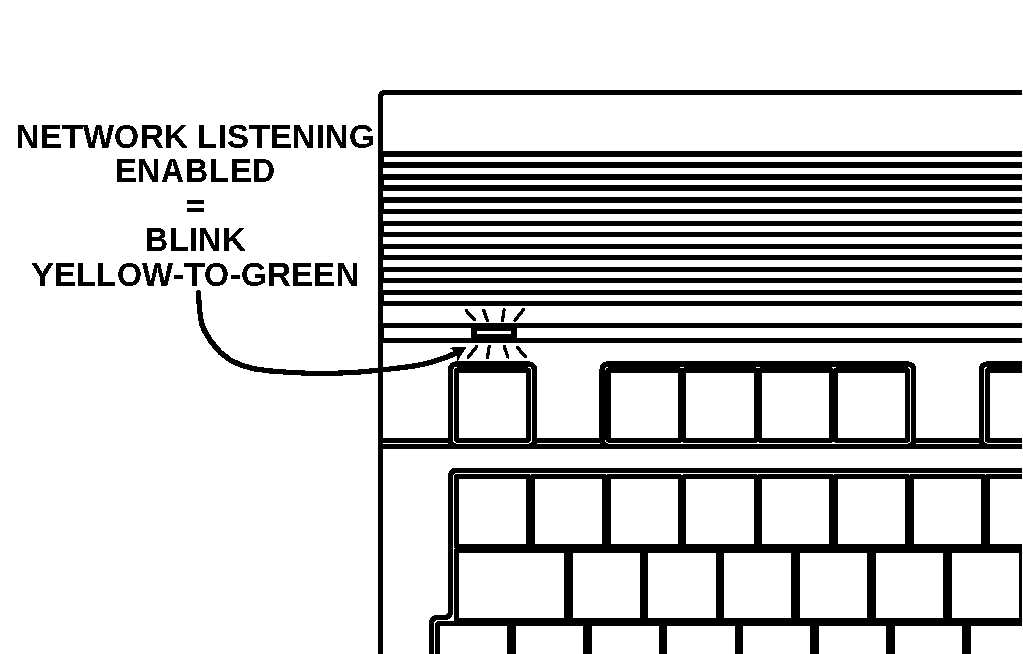
\includegraphics[width=\linewidth]{images/illustrations/mega65-eth-blink.pdf}
\end{center}

\underline{Note}: Resetting the computer disables network listening. Press \specialkey{SHIFT} + \megakey{\pounds} to start a new session.

\section{Transferring Files}

To transfer files, you will start a file transfer session using the M65Connect application or the {\tt mega65\_ftp} command-line tool. This connects to the MEGA65 and uploads a file transfer client for use during the session. When you end the session, the MEGA65 resets.

Starting a file transfer session resets the MEGA65. As a precaution, the session will not start if there is a program in memory. Save any programs or data, then clear program memory (such as with the {\bf NEW} command) before proceeding.

\underline{Note}: If you clear memory by resetting the computer, remember to re-enable network listening: press \specialkey{SHIFT} + \megakey{\pounds}, and ensure the power light is blinking.

\subsection{Transferring Files with M65Connect}
\index{M65Connect Application}

(This section is pending the release of a new version of M65Connect.)

% TODO: These instructions are pending an update to M65Connect that implements this procedure.

\subsection{The mega65\_ftp Command-Line Tool}
\index{mega65\_ftp command@\texttt{mega65\_ftp command}}

The {\tt mega65\_ftp} command-line tool initiates a file transfer session with the MEGA65. It can run interactively in the terminal and accept multiple file transfer commands, or it can run non-interactively with those commands provided as arguments.

% TODO: This may be updated in the future to allow for automatic selection of an IP address.

To start an interactive file transfer session, run the {\tt mega65\_ftp} command, providing the IP address you have selected for the MEGA65 as the {\tt -i} argument.

\begin{verbatim}
% mega65_ftp -i 192.168.0.65
\end{verbatim}

The tool will upload the file transfer client, and you will see it the client running on the MEGA65. If nothing happens, press Ctrl-C (on the PC) to abort, then double-check that the MEGA65 is connected and that network listening is enabled.

Once connected, the file transfer command prompt looks similar to this:

\begin{verbatim}
MEGA65 SD-Card:/>
\end{verbatim}

To end the session, use the {\tt exit} command. The tool will exit and return to the shell prompt, and the MEGA65 will reset.

\begin{verbatim}
MEGA65 SD-Card:/> exit
%
\end{verbatim}

The following are several useful commands you can use during the file transfer session. Use the {\tt help} command to see a complete list of available commands.

\begin{center}
\begin{tabular}{|l|l|}
\hline
{\bf Command} & {\bf Description} \\
\hline
{\tt put {\it filename}} & Send a file from the PC to the MEGA65. \\
\hline
{\tt get {\it filename}} & Retrieve a file from the MEGA65 to the PC. \\
\hline
{\tt dir} & Display a directory listing of the MEGA65 SD card. \\
\hline
{\tt ldir} & Display a directory listing of the local current working directory. \\
\hline
{\tt mkdir {\it dirname}} & Create a sub-directory on the MEGA65 SD card. \\
\hline
{\tt cd {\it dirname}} & Change the current working directory on the MEGA65 SD card. \\
\hline
{\tt help} & Display a list of available commands. \\
\hline
{\tt exit} & End the file transfer session. \\
\hline
\end{tabular}
\end{center}

To invoke {\tt mega65\_ftp} commands without starting an interactive prompt, use the {\tt -c} argument once for each command:

\begin{verbatim}
% mega65_ftp -i 192.168.0.65 -c 'put mydisk.d81' -c 'exit'
\end{verbatim}

The tool will start a session, execute the commands, then terminate. Be sure to issue the {\tt exit} command as the final command to reset the MEGA65, or reset the MEGA65 manually after the file transfer has completed.